\documentclass[12pt]{beamer}

\usepackage[english]{babel}
\usepackage[utf8]{inputenc}
\usepackage{tikz}

\usetheme{Copenhagen}

\title{Category Jaccard averaged on the Outlinks}
\author[Jacopo Notarstefano]{
    Jacopo Notarstefano\\
    \texttt{jacopo.notarstefano [at] gmail.com}
}
\date{11 February 2014}

\begin{document}
    \begin{frame}[plain]
        \titlepage
    \end{frame}

    \begin{frame}{Category Jaccard}
        \begin{definition}[Category Jaccard]
            Let \(p_1\) and \(p_2\) be two pages and let \(C_1\) and \(C_2\)
            be, respectively, their list of categories. Then their Category
            Jaccard similarity is
            \[
                J_C(p_1, p_2) = \frac{|C_1\cap C_2|}{|C_1\cup C_2|}\text{.}
            \]
        \end{definition}
    \end{frame}

    \begin{frame}{Category Jaccard averaged on the Outlinks}
        \begin{definition}[Category Jaccard averaged on the Outlinks]
            Let \(p_1\) and \(p_2\) be two pages and let \(O^1\) and \(O^2\) be,
            respectively, their list of linked pages. Then their
            Category Jaccard similarity averaged on the Outlinks is
            \[
                \text{AVG}_{J_C}(p_1, p_2) = \frac{\sum{J_C(O^1_i, O^2_j)}}{|O^1|\cdot|O^2|}\text{.}
            \]
        \end{definition}
    \end{frame}


    \begin{frame}{A picture \(\approx 2^{10}\) words}
        \begin{figure}
            \centering
            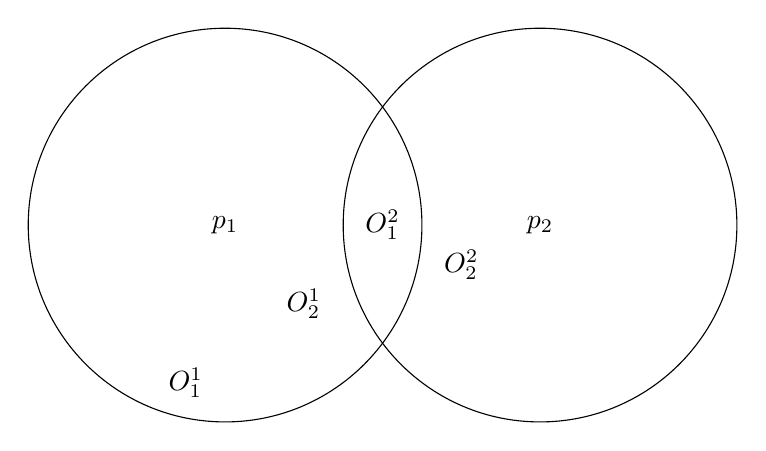
\begin{tikzpicture}
                \node (p1) at (3,2) [] {$p_1$};
                \node (p2) at (7,2) [] {$p_2$};
                \node (c1) at (3,2) [circle,draw=black!100,minimum size=5cm] {};
                \node (c2) at (7,2) [circle,draw=black!100,minimum size=5cm] {};

                \node (o11) at (2.5,0) [] {$O^1_1$};
                \node (o12) at (4,1) [] {$O^1_2$};
                \node (o13) at (5,2) [] {$O^2_1$};
                \node (o22) at (6,1.5) [] {$O^2_2$};
            \end{tikzpicture}
        \end{figure}
    \end{frame}

    \begin{frame}{Advantages}
    \end{frame}

    \begin{frame}{Drawbacks}
    \end{frame}
\end{document}
